\documentclass[10pt, xcolor=dvipsnames]{beamer}

%PTBR
%\usepackage[brazilian]{babel}
\usepackage[utf8]{inputenc}
\usepackage[T1]{fontenc}
\usepackage{bm}
\usepackage{graphicx}
\usepackage[absolute,overlay]{textpos} %pacote para posicionar o logo na primeira página

\usetheme[progressbar=frametitle]{metropolis}
\usepackage{appendixnumberbeamer}

\usepackage{booktabs}
\usepackage[scale=2]{ccicons}

\usepackage{pgfplots}
\usepgfplotslibrary{dateplot}

\usepackage{xspace}
\newcommand{\themename}{\textbf{\textsc{metropolis}}\xspace}

\usepackage{MacrosSlides}
\usetikzlibrary{arrows.meta} %TIKZ
%\usetikzlibrary{tikzmark} %Arrows over tables (?)
\usetikzlibrary{shapes.misc, positioning}

%%% \bigsqcap -- stack exchange
\makeatletter
\providecommand{\bigsqcap}{%
  \mathop{%
    \mathpalette\@updown\bigsqcup
  }%
}
\newcommand*{\@updown}[2]{%
  \rotatebox[origin=c]{180}{$\m@th#1#2$}%
}
\makeatother

%\definecolor{teal}{rgb}{0.0, 0.5, 0.5}
%\definecolor{darkRedOrange}{rgb}{1.0, 0.55, 0.0}

\title{Quantification in Description Logics of Typicality}

\titlegraphic{%
  \begin{picture}(0,0)
    \put(305,-120){\makebox(0,0)[rt]{\includegraphics[width=6cm]{img/ime_logo.png}}}
  \end{picture}}

\date{July 18th 2023}
\author{Igor de Camargo e Souza Câmara}
\institute{University of São Paulo}


\begin{document}

\begin{frame}[plain]
  \titlepage
\end{frame}

%
% 1. Outline and motivation
%

\begin{frame}[fragile]{Outline}
  \large
  \begin{itemize}
    \item Extend Description Logics (DLs) with reasoning inspired by the prototype theory of conceptualization.
    \item Several suggestions in the literature are based on propositional settings.
    \item Falling short of dealing with DL's first-order nature.
    \item We examine a new semantical framework -- typicality models -- to deal with quantified defeasible inference. 
  \end{itemize}
\end{frame}

\begin{frame}[fragile]{Motivation}
\large
DLs represent concepts by \emph{list of necessary sufficient conditions}.

\begin{enumerate}
  \item A Trojan soldier is a soldier natural from Troy.
  \begin{itemize}
    \item $\dlFont{TrojanSoldier} \sqsubseteq \dlFont{Human} \sqcap \dlFont{Trojan} \sqcap \dlFont{Soldier}$
  \end{itemize} \pause
  \item A parent is someone who is the father or the mother to someone.
  \begin{itemize}
    \item $\dlFont{Parent} \sqsubseteq \exists \dlFont{fatherOf}.\top \sqcup \dlFont{Parent} \sqsubseteq \exists \dlFont{motherOf}.\top$
  \end{itemize}
\end{enumerate}
\end{frame}

\begin{frame}[fragile]{Motivation}
  \large
  Prototype theory presents an alternate theory of conceputalization.

  \begin{itemize}
    \item Similarity between recognized members.
    \item Different grades of membership.
    \item Ideal concept members, \ie prototypes.
  \end{itemize}
\end{frame}
  
\begin{frame}[fragile]{Motivation}
\includegraphics[scale=.33]{img/birdstyp.png}
\end{frame}

\begin{frame}[fragile]{Motivation}
  \includegraphics[scale=.33]{img/familyres.png}
\end{frame}

% Speak: the idea is to incorporate prototype reasoning through defeasible reasoning.

%
% 2. DDLs and Materialization
%

\begin{frame}{Defeasible Knowledge Bases}
  \begin{center}
    \Large{
      $\Kmc = ({\color{Plum}\Amc}, {\color{RedOrange} \Tmc}, {\color{teal} \Dmc})$
    }
  \end{center}

  \bigskip

  \begin{columns}[t,onlytextwidth]

    \column{.3\textwidth} 
  {\color{Plum} $\dlFont{Human}({hector})$} \\ 
  {\color{Plum} $\dlFont{Deity}({athena})$}
  
  \column{.3\textwidth} 
  {\color{RedOrange} $\dlFont{Deity} \sqsubseteq \dlFont{Being}$} \\
  {\color{RedOrange} $\dlFont{Deity} \sqcap \dlFont{Mortal} \sqsubseteq \bot$} \\
  {\color{RedOrange} $\dlFont{Human} \sqsubseteq \dlFont{Being}$} 
  \vspace{2mm}

  \column{.4\textwidth} 
  {\color{teal} $\dlFont{Being} \definc \dlFont{Mortal}$} \\
  {\color{teal} $\dlFont{Being} \definc \dlFont{Corporeal}$} \\
  {\color{teal} $\dlFont{Human} \definc \dlFont{\exists \dlFont{worship}.\dlFont{Deity}}$} \\
  {\color{teal} $\dlFont{Deity} \definc \dlFont{Anthropomorphic}$}
  \vspace{2mm}

  \end{columns}
\end{frame}

\begin{frame}{Materialization-based Reasoning}

\textbf{Materialisation} \\
$\materialization{C \definc D} \Rightarrow \lnot C \sqcup D$ \\
$\materialization{\Umc} = \bigsqcap_{C \definc D \in \Umc} \materialization{C \definc D}$
\medskip

\textbf{Materialisation-based Defeasible Subsumption Checking} \\
$\Kmc \models C \definc D \text{ iff } \Kmc \models C \sqcap \materialization{\Umc} \sqsubseteq D$
for some $\Umc \subseteq \Dmc$ \medskip

\textbf{Rational Chain} \\
$\Dmc = \Emc_0 \supset \Emc_1 \supset \dots \supset \Emc_n$
\end{frame}

\begin{frame}{Rational Reasoning}
  \begin{tikzpicture}

    % 
    \draw[gray,thick,fill=gray!30,rounded corners] (0, 3) rectangle (4,6); %TBox
        \node[] at (2, 6.4) (TBox) {{\Large $\Tmc$}};

    \draw[gray,thick,fill=gray!30,rounded corners] (4.5, 2) rectangle (9.5,6); %DBox E_0
        \node[] at (7, 6.4) (DBox) {{\Large $\Dmc = \Emc_0$}};

    \draw[gray,thick,fill=gray!30,rounded corners] (4.7, 5) rectangle (9.3,5.8); %DBox E_1
        \node[] at (10, 5.4) (DBox) {{\Large $\Emc_1$}};

    % T - Axioms
    \node [] at (2, 4.5) (TAxiom) {\begin{tabular}{c} {\large $\dlFont{Deity} \sqsubseteq \dlFont{Being}$} \\ ~ \\ {\large $\dlFont{Human} \sqsubseteq \dlFont{Being}$}  \\ ~ \\ {\large $\dlFont{Deity} \sqcap \dlFont{Mortal} \sqsubseteq \bot$} \end{tabular}};

    % E_0 - Axioms
    \node [] at (7, 5.5) (E_0Axiom) {\large $\dlFont{Deity} \definc \dlFont{Anthropomorphic}$};

    % E_1 - Axioms
    \node [] at (7, 3.5) (E_1Axiom) {\begin{tabular}{c} {\large $\dlFont{Being} \definc \dlFont{Mortal}$} \\ ~ \\ {\large $\dlFont{Being} \definc \dlFont{Corporeal}$} \\ ~ \\ {\large $\dlFont{Human} \sqsubseteq \exists \dlFont{worships}.\dlFont{Deity}$} \end{tabular}};        

    \end{tikzpicture}
\end{frame}

\begin{frame}{Rational Reasoning}
  \begin{tikzpicture}

    % 
    \draw[gray,thick,fill=gray!30,rounded corners] (0, 3) rectangle (4,6); %TBox
        \node[] at (2, 6.4) (TBox) {{\Large $\Tmc$}};

    \draw[gray,thick,fill=gray!30,rounded corners] (4.5, 2) rectangle (9.5,6); %DBox E_0
        \node[] at (7, 6.4) (DBox) {{\Large $\Dmc = \Emc_0$}};

    \draw[Plum,thick,fill=Plum!50,rounded corners] (4.7, 5) rectangle (9.3,5.8); %TBox
        \node[] at (10, 5.4) (DBox) {{\color{Plum} \Large $\Emc_1$}};

    % T - Axioms
    \node [] at (2, 4.5) (TAxiom) {\begin{tabular}{c} {\large $\dlFont{Deity} \sqsubseteq \dlFont{Being}$} \\ ~ \\ {\large $\dlFont{Human} \sqsubseteq \dlFont{Being}$}  \\ ~ \\ {\large $\dlFont{Deity} \sqcap \dlFont{Mortal} \sqsubseteq \bot$} \end{tabular}};

    % E_0 - Axioms
    \node [] at (7, 5.5) (E_0Axiom) {\large $\dlFont{Deity} \definc \dlFont{Anthropomorphic}$};

    % E_1 - Axioms
    \node [] at (7, 3.5) (E_1Axiom) {\begin{tabular}{c} {\large $\dlFont{Being} \definc \dlFont{Mortal}$} \\ ~ \\ {\large $\dlFont{Being} \definc \dlFont{Corporeal}$} \\ ~ \\ {\large $\dlFont{Human} \definc\exists \dlFont{worships}.\dlFont{Deity}$} \end{tabular}};        
    \end{tikzpicture}

    \medskip 

    \begin{center}
    {\large$\Kmc \not\models \dlFont{Deity} \definc \dlFont{Corporeal}$}
    \end{center}
\end{frame}

\begin{frame}{Rational Reasoning}
  \begin{tikzpicture}

    % 
    \draw[gray,thick,fill=gray!30,rounded corners] (0, 3) rectangle (4,6); %TBox
        \node[] at (2, 6.4) (TBox) {{\Large $\Tmc$}};

    \draw[Plum,thick,fill=Plum!50,rounded corners] (4.5, 2) rectangle (9.5,6); %DBox E_0
        \node[] at (7, 6.4) (DBox) {{\color{Plum} \Large $\Dmc = \Emc_0$}};

    \draw[Plum!50,thick,fill=Plum!50,rounded corners] (4.7, 5) rectangle (9.3,5.8); %TBox
        \node[] at (10, 5.4) (DBox) {{\Large $\Emc_1$}};

    % T - Axioms
    \node [] at (2, 4.5) (TAxiom) {\begin{tabular}{c} {\large $\dlFont{Deity} \sqsubseteq \dlFont{Being}$} \\ ~ \\ {\large $\dlFont{Human} \sqsubseteq \dlFont{Being}$}  \\ ~ \\ {\large $\dlFont{Deity} \sqcap \dlFont{Mortal} \sqsubseteq \bot$} \end{tabular}};

    % E_0 - Axioms
    \node [] at (7, 5.5) (E_0Axiom) {\large $\dlFont{Deity} \definc \dlFont{Anthropomorphic}$};

    % E_1 - Axioms
    \node [] at (7, 3.5) (E_1Axiom) {\begin{tabular}{c} {\large $\dlFont{Being} \definc \dlFont{Mortal}$} \\ ~ \\ {\large $\dlFont{Being} \definc \dlFont{Corporeal}$} \\ ~ \\ {\large $\dlFont{Human} \definc\exists \dlFont{worships}.\dlFont{Deity}$} \end{tabular}};        
    \end{tikzpicture}

    \medskip 

    \begin{center}
    {\large$\Kmc \models \dlFont{Human} \definc \dlFont{Mortal}$}
    \end{center}
\end{frame}

\begin{frame}{Quantification Neglect in Rational Reasoning}
  \begin{tikzpicture}

    % 
    \draw[gray,thick,fill=gray!30,rounded corners] (0, 3) rectangle (4,6); %TBox
        \node[] at (2, 6.4) (TBox) {{\Large $\Tmc$}};

    \draw[Plum,thick,fill=Plum!50,rounded corners] (4.5, 2) rectangle (9.5,6); %DBox E_0
        \node[] at (7, 6.4) (DBox) {{\color{Plum} \Large $\Dmc = \Emc_0$}};

    \draw[Plum!50,thick,fill=Plum!50,rounded corners] (4.7, 5) rectangle (9.3,5.8); %TBox
        \node[] at (10, 5.4) (DBox) {{\Large $\Emc_1$}};

    % T - Axioms
    \node [] at (2, 4.5) (TAxiom) {\begin{tabular}{c} {\large $\dlFont{Deity} \sqsubseteq \dlFont{Being}$} \\ ~ \\ {\large $\dlFont{Human} \sqsubseteq \dlFont{Being}$}  \\ ~ \\ {\large $\dlFont{Deity} \sqcap \dlFont{Mortal} \sqsubseteq \bot$} \end{tabular}};

    % E_0 - Axioms
    \node [] at (7, 5.5) (E_0Axiom) {\large $\dlFont{Deity} \definc \dlFont{Anthropomorphic}$};

    % E_1 - Axioms
    \node [] at (7, 3.5) (E_1Axiom) {\begin{tabular}{c} {\large $\dlFont{Being} \definc \dlFont{Mortal}$} \\ ~ \\ {\large $\dlFont{Being} \definc \dlFont{Corporeal}$} \\ ~ \\ {\large $\dlFont{Human} \definc\exists \dlFont{worships}.\dlFont{Deity}$} \end{tabular}};        
    \end{tikzpicture}

    \medskip 

    \begin{center}
    {\large$\Kmc \not\models \dlFont{Human} \definc \exists \dlFont{worships}.\dlFont{Anthropomorphic}$}
    \end{center}
\end{frame}

%
% 3. Typicality Models -- Intro
%

\begin{frame}{Typicality Models -- Outline}
\large
\begin{itemize}
  \item Special interpretations based on canonical models for lightweigth DLs.
  \item Define satisfaction for defeasible concept inclusion.
  \item By constraining the domain, it is possible to achieve canonical models for several materialization-based reasoning procedures.
\end{itemize}
\end{frame}

\begin{frame}{Typicality Models -- The Basics}
  \begin{center}
    \Large{
      $\typel{\color{Plum}C}{\color{RedOrange}\Umc}$
    }
  \end{center}

  {\color{Plum}$C$} represents a concept and ${\color{RedOrange}\Umc} \subseteq \Dmc$ is a set of DCIs.

  Typicality interpretation is an interpretation $\Imc = (\Delta^{\Imc}, \cdot^{\Imc})$.

  \medskip \pause

  \textbf{Satisfaction}

  \begin{itemize}
    \item $\Imc \models C \sqsubseteq D$ iff $C^{\Imc} \subseteq D^{\Imc}$
    \item $\Imc \models C \definc D$ iff $\typel{C}{\Umc} \in D^{\Imc}$ for maximally typical $\typel{C}{\Umc}$.
  \end{itemize}

% COMMENT: pure entailment does not interest us. Only 'flavored' (i.e. prop/nest x rat/rel/lex)

\end{frame}

\begin{frame}{Propositional and Nested Entailments}
\large 
\begin{itemize}
  \item Entailment is parametrized along two axis: \textbf{strength} and \textbf{coverage}.
  \item Strength refers to the materialization-based procedure and is defined by the shape of the domain.
  \item Coverage refers to the quantification depth of defeasible information.
\end{itemize}
$$\{\ratS, \relS, \lexS\} \times \{\propCov, \nestCov\}$$
\end{frame}

\begin{frame}{Typicality Domain in $\ELbot$ and $\ELIbot$}

    {\color{Plum}
    \large{(\ELbot)} \large{$C \sqsubseteq \exists r.D \Rightarrow (C,D) \in r^{\minrattypp}$}}

\medskip \pause

{\large $\Tmc = \{ A \sqsubseteq \exists r.B, A \sqsubseteq \forall r.C \}$}

\medskip \pause

  \centering{
  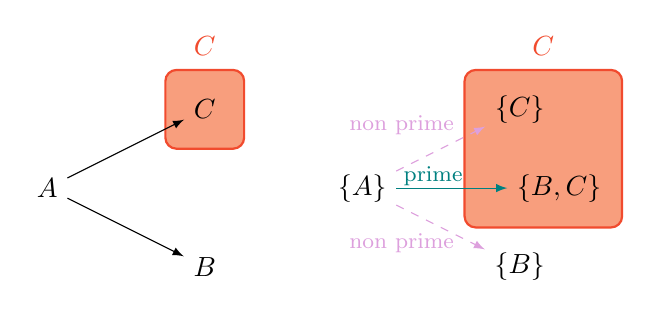
\begin{tikzpicture}
    \draw[RedOrange,thick,fill=RedOrange!50,rounded corners] (1.5, 1.5) rectangle (2.5,2.5); %C Concept
      \node[] at (2,2.8) (CCon) {{\color{RedOrange}$C$}};

    \node[] at (0,1) (A) {$A$};
    \node[] at (2,0) (B) {$B$};
    \node[] at (2,2) (C) {$C$};

    \draw[-latex](A) to (B);
    \draw[-latex](A) to (C);

    \pause

    \draw[RedOrange,thick,fill=RedOrange!50,rounded corners] (5.3, 0.5) rectangle (7.3,2.5);
      \node[] at (6.3,2.8) (CCon) {{\color{RedOrange}$C$}};

    \node[] at (4,1) (A2) {$\{A\}$};
    \node[] at (6,0) (B2) {$\{B\}$};
    \node[] at (6,2) (C2) {$\{C\}$};
    \node[] at (6.5,1) (BC) {$\{B,C\}$};

    \draw[-latex, color=teal](A2) to (BC);

    \draw[-latex, color=Plum, dashed](A2) to (C2);
    \draw[-latex, color=Plum, dashed](A2) to (B2);

    \node[] at (4.9,1.15) (CCon) {{\footnotesize \color{teal}prime}};

    \node[] at (4.5,1.8) (CCon) {{\footnotesize \color{Plum}non prime}};
    \node[] at (4.5,0.3) (CCon) {{\footnotesize \color{Plum}non prime}};

    %\node[] at (3.5, -1) (text) {\large $C \sqsubseteq \exists r.M$ \textbf{ and } $M$ \text{ is maximal } \wrt $\Kmc, C, r \Rightarrow (C,M) \in r^{\minrattypp}$ };
  \end{tikzpicture}}

  \medskip \pause

  Concept set contains:
\begin{enumerate}
  \item Singletons of named concepts and 
  \item Combinations of named concepts occurring within quantifiers.
\end{enumerate}
\end{frame}

\begin{frame}{Minimal Typicality Model}

  $\dlFont{Human} \sqsubseteq \forall \dlFont{worships}.\dlFont{Powerful}$
  \medskip

  \centering{
  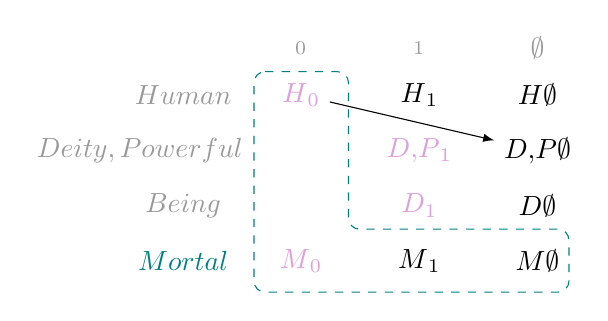
\begin{tikzpicture}
    %\draw[dashed] (1, 3) rectangle (5, 0.3);

    \draw[dashed, teal, rounded corners] (0.9, 3) -- (2.1, 3) -- (2.1,2.3) -- (2.1, 1) -- (4.9, 1) -- (4.9, 0.2) -- (0.9, 0.2) -- cycle;

    \node[color=black!40] at (0, 1.3){$\dlFont{Being}$};
    \node[color=black!40] at (0, 2.7){$\dlFont{Human}$};
    \node[color=black!40] at (-0.55, 2){$\dlFont{Deity}, \dlFont{Powerful}$};
    \node[color=teal] at (0, 0.6){$\dlFont{Mortal}$};

    \node[color=black!40] at (1.5,3.3){$\Emc_0$};
    \node[color=black!40] at (3,3.3){$\Emc_1$};
    \node[color=black!40] at (4.5,3.3){$\emptyset$};
    
    \node[Plum] at (3,1.3){$\typel{\dlFont{D}}{\Emc_{1}}$};
    \node[] at (4.5,1.3){$\typel{\dlFont{D}}{\emptyset}$};

    \node[Plum] (H2) at (1.5, 2.7){$\typel{\dlFont{H}}{\Emc_{0}}$};
    \node[] (H1) at (3, 2.7){$\typel{\dlFont{H}}{\Emc_{1}}$};
    \node[] (H0) at (4.5, 2.7){$\typel{\dlFont{H}}{\emptyset}$};

    %\node[Plum] at (1.5,2){$\typel{\dlFont{D,P}}{\Emc_{0}}$};
    \node[Plum] (DP1) at (3,2){$\typel{\dlFont{D},\!\dlFont{P}}{\Emc_{1}}$};
    \node[] (DP0) at (4.5,2){$\typel{\dlFont{D},\!\dlFont{P}}{\emptyset}$};

    \node[Plum] at (1.5,0.6){$\typel{\dlFont{M}}{\Emc_{0}}$};
    \node[] at (3,0.6){$\typel{\dlFont{M}}{\Emc_{1}}$};
    \node[] at (4.5,0.6){$\typel{\dlFont{M}}{\emptyset}$};

    %\draw[-latex] (H0) -- (5.5, 2.35) -- (DP0);
    %\draw[-latex] (H1) -- (DP0);
    \draw[-latex] (H2) -- (DP0);

    \node[] at (0.3,3.4){$\footnotesize \ratDom$};
\end{tikzpicture} 
  }

\bigskip 

\begin{enumerate}
  \item $\typel{M}{\Umc} \in A^{\Mintypmod}$ iff $\materialization{\Kmc} \models \setconj{M} \sqcap \materialization{\Umc} \sqsubseteq A$
  \item $(\typel{M}{\Umc}, \typel{N}{\Vmc}) \in r^{\Mintypmod}$ iff $\materialization{\Kmc} \models \setconj{M} \sqcap \materialization{\Umc} \sqsubseteq \exists r.\setconj{N}$ and $N$ is prime.
\end{enumerate}

\end{frame}

\begin{frame}{Lattice Domains -- Relevant and Lexicographic}

  \centering{
    \scalebox{.95}{
          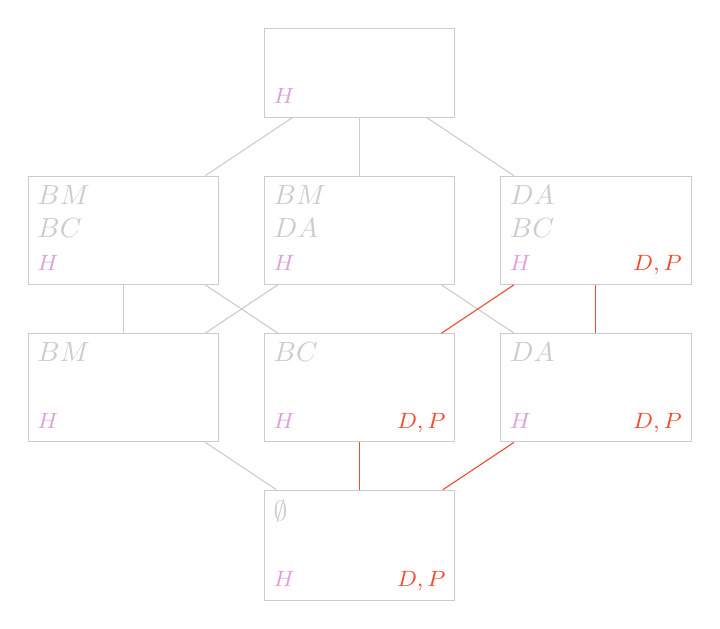
\begin{tikzpicture}
              \node[align=left, draw, color=black!20] at (0,6) (D) {\color{black!20}$\Dmc$  \\ \color{white}$\dlFont{C} \definc \dlFont{F} \hspace{8mm}$ \\ \footnotesize {\color{Plum}$\dlFont{H} \hspace{12mm}$}{ \color{white} $\dlFont{D,P}$}};
            
              %%% Level 2
            
              \node[align=left, draw, color=black!20] at (-3,4) (B1B2) {\color{black!20}$\dlFont{B} \definc \dlFont{M}$  \\ \color{black!20}$\dlFont{B} \definc \dlFont{C} \hspace{8mm}$ \\ \footnotesize {\color{Plum}$\dlFont{H} \hspace{12mm}$}{ \color{white} $\dlFont{D,P}$}};
            
              \node[align=left, draw, color=black!20] at (0,4) (B1P) {\color{black!20}$\dlFont{B} \definc \dlFont{M}$ \\ \color{black!20}$\dlFont{D} \definc \dlFont{A}$ \\ \footnotesize {\color{Plum}$\dlFont{H} \hspace{12mm}$}{ \color{white} $\dlFont{D,P}$}};
            
              \node[align=left, draw, color=black!20] at (3,4) (B2P) {\color{black!20}$\dlFont{D} \definc \dlFont{A} \hspace{8mm}$ \\ \color{black!20}$\dlFont{B} \definc \dlFont{C}$ \\ \footnotesize {\color{Plum}$\dlFont{H} \hspace{12mm}$}{ \color{RedOrange} $\dlFont{D,P}$}};
            
              %%% Level 1
            
              \node[align=left, draw, color=black!20] at (-3,2) (B1) {\color{black!20}$\dlFont{B} \definc \dlFont{M}$  \\ \color{white}$\dlFont{C} \definc \dlFont{F} \hspace{8mm}$ \\\footnotesize {\color{Plum}$\dlFont{H} \hspace{12mm}$}{ \color{white} $\dlFont{D,P}$}};
            
              \node[align=left, draw, color=black!20] at (0,2) (B2) {\color{black!20}$\dlFont{B} \definc \dlFont{C}$ \\ \color{white}$\dlFont{D} \definc \dlFont{I}$ \\ \footnotesize {\color{Plum}$\dlFont{H} \hspace{12mm}$}{ \color{RedOrange} $\dlFont{D,P}$}};
            
              \node[align=left, draw, color=black!20] at (3,2) (P) {\color{black!20}$\dlFont{D} \definc \dlFont{A}$ \\ \color{white}$\dlFont{C} \definc \dlFont{F}$ \\ \footnotesize {\color{Plum}$\dlFont{H} \hspace{12mm}$}{ \color{RedOrange} $\dlFont{D,P}$}};
            
              %%%% Level 0
            
              \node[align=left, draw, color=black!20] at (0,0) (empty) {\color{black!20}$\emptyset$ \\ \color{white}$\dlFont{C} \definc \dlFont{F} \hspace{8mm}$ \\ \footnotesize {\color{Plum}$\dlFont{H} \hspace{12mm}$}{ \color{RedOrange} $\dlFont{D,P}$}};
              
              %%% Lattice lines
              \draw[-, color=black!20] (D)--(B1B2);
              \draw[-, color=black!20] (D)--(B1P);
              \draw[-, color=black!20] (D)--(B2P);
            
              \draw[-, color=black!20] (B1B2)--(B1);
              \draw[-, color=black!20] (B1B2)--(B2);
            
              \draw[-, color=black!20] (B1P)--(B1);
              \draw[-, color=black!20] (B1P)--(P);
            
              \draw[-, color=RedOrange] (B2P)--(B2);
              \draw[-, color=RedOrange] (B2P)--(P);
            
              \draw[-, color=black!20] (B1)--(empty);
              \draw[-, color=RedOrange] (B2)--(empty);
              \draw[-, color=RedOrange] (P)--(empty);
            
              %\draw[-latex, thick, bend left] (-0.7,5.5) to(3.8,3.6);
            
              \end{tikzpicture}
           }
        }

\end{frame}

\begin{frame}{Propositional Reasoning}

\begin{itemize}
  \item Propositional \strength-reasoning is defined by the minimal typicality model with \strength-domain.
  \begin{enumerate}
    \item $\Kmc \modelsprop{\strength} \setconj{M} \sqsubseteq A$ \emph{ iff } $\mintypmod \models \setconj{M} \sqsubseteq A$
    \item $\Kmc \modelsprop{\strength} \setconj{M} \definc A$ \emph{ iff } $\mintypmod \models \setconj{M} \definc A$
\end{enumerate}
\end{itemize}

\medskip \pause 

\centering{
  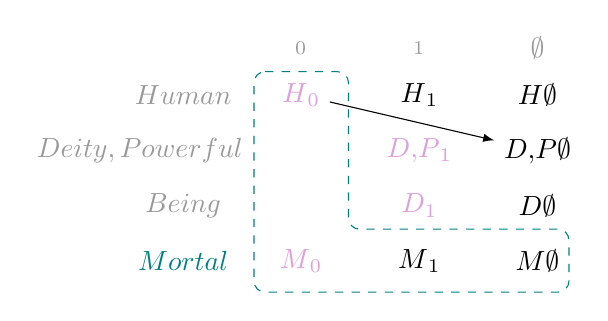
\begin{tikzpicture}
    %\draw[dashed] (1, 3) rectangle (5, 0.3);

    \draw[dashed, teal, rounded corners] (0.9, 3) -- (2.1, 3) -- (2.1,2.3) -- (2.1, 1) -- (4.9, 1) -- (4.9, 0.2) -- (0.9, 0.2) -- cycle;

    \node[color=black!40] at (0, 1.3){$\dlFont{Being}$};
    \node[color=black!40] at (0, 2.7){$\dlFont{Human}$};
    \node[color=black!40] at (-0.55, 2){$\dlFont{Deity}, \dlFont{Powerful}$};
    \node[color=teal] at (0, 0.6){$\dlFont{Mortal}$};

    \node[color=black!40] at (1.5,3.3){$\Emc_0$};
    \node[color=black!40] at (3,3.3){$\Emc_1$};
    \node[color=black!40] at (4.5,3.3){$\emptyset$};
    
    \node[Plum] at (3,1.3){$\typel{\dlFont{D}}{\Emc_{1}}$};
    \node[] at (4.5,1.3){$\typel{\dlFont{D}}{\emptyset}$};

    \node[Plum] (H2) at (1.5, 2.7){$\typel{\dlFont{H}}{\Emc_{0}}$};
    \node[] (H1) at (3, 2.7){$\typel{\dlFont{H}}{\Emc_{1}}$};
    \node[] (H0) at (4.5, 2.7){$\typel{\dlFont{H}}{\emptyset}$};

    %\node[Plum] at (1.5,2){$\typel{\dlFont{D,P}}{\Emc_{0}}$};
    \node[Plum] (DP1) at (3,2){$\typel{\dlFont{D},\!\dlFont{P}}{\Emc_{1}}$};
    \node[] (DP0) at (4.5,2){$\typel{\dlFont{D},\!\dlFont{P}}{\emptyset}$};

    \node[Plum] at (1.5,0.6){$\typel{\dlFont{M}}{\Emc_{0}}$};
    \node[] at (3,0.6){$\typel{\dlFont{M}}{\Emc_{1}}$};
    \node[] at (4.5,0.6){$\typel{\dlFont{M}}{\emptyset}$};

    %\draw[-latex] (H0) -- (5.5, 2.35) -- (DP0);
    %\draw[-latex] (H1) -- (DP0);
    \draw[-latex] (H2) -- (DP0);

    \node[] at (0.3,3.4){$\footnotesize \ratDom$};
\end{tikzpicture} 
  }

  \medskip 

  \begin{columns}[t,onlytextwidth]

    \column{.5\textwidth} 
  {\footnotesize
  \begin{itemize}
    \item $\Kmc \models \dlFont{Human} \definc \exists \dlFont{worships}.\dlFont{Powerful}$
    \item $\Kmc \models \dlFont{Human} \definc \dlFont{Mortal}$
  \end{itemize}
  }
\pause
  \column{.6\textwidth}
  {\footnotesize
  \begin{itemize}
    \item $\color{red} \Kmc \not\models \dlFont{Human} \definc \exists \dlFont{worships}.\dlFont{Anthropomorphic}$
    \item $\color{red} \Kmc \not\models \dlFont{Deity} \definc \dlFont{Corporeal}$
  \end{itemize}
  }

\end{columns}
\end{frame}

\begin{frame}{Nested Reasoning -- Outline}

  \centering{
    \begin{tikzpicture}
      %\draw[dashed] (1, 3) rectangle (5, 0.3);
  
      \draw[dashed, black!40, rounded corners] (0.9, 3) -- (2.1, 3) -- (2.1,2.3) -- (2.1, 1) -- (4.9, 1) -- (4.9, 0.2) -- (0.9, 0.2) -- cycle;
  
      \node[color=black!40] at (0, 1.3){$\dlFont{Being}$};
      \node[color=black!40] at (0, 2.7){$\dlFont{Human}$};
      \node[color=black!40] at (-0.55, 2){$\dlFont{Deity}, \dlFont{Powerful}$};
      \node[color=black!40] at (0, 0.6){$\dlFont{Mortal}$};
  
      \node[color=black!40] at (1.5,3.3){$\Emc_0$};
      \node[color=black!40] at (3,3.3){$\Emc_1$};
      \node[color=black!40] at (4.5,3.3){$\emptyset$};
      
      \node[black!40] at (3,1.3){$\typel{\dlFont{D}}{\Emc_{1}}$};
      \node[black!40] at (4.5,1.3){$\typel{\dlFont{D}}{\emptyset}$};
  
      \node[Plum] (H2) at (1.5, 2.7){$\typel{\dlFont{H}}{\Emc_{0}}$};
      \node[black!40] (H1) at (3, 2.7){$\typel{\dlFont{H}}{\Emc_{1}}$};
      \node[black!40] (H0) at (4.5, 2.7){$\typel{\dlFont{H}}{\emptyset}$};
  
      %\node[Plum] at (1.5,2){$\typel{\dlFont{D,P}}{\Emc_{0}}$};
      \node[black!40] (DP1) at (3,2){$\typel{\dlFont{D},\!\dlFont{P}}{\Emc_{1}}$};
      \node[Plum] (DP0) at (4.5,2){$\typel{\dlFont{D},\!\dlFont{P}}{\emptyset}$};
  
      \node[black!40] at (1.5,0.6){$\typel{\dlFont{M}}{\Emc_{0}}$};
      \node[black!40] at (3,0.6){$\typel{\dlFont{M}}{\Emc_{1}}$};
      \node[black!40] at (4.5,0.6){$\typel{\dlFont{M}}{\emptyset}$};
  
      %\draw[-latex] (H0) -- (5.5, 2.35) -- (DP0);
      %\draw[-latex] (H1) -- (DP0);
      \draw[-latex, Plum] (H2) -- (DP0);
  
      \node[black!40] at (0.3,3.4){$\footnotesize \ratDom$};

      \pause 

      \draw[-latex, RedOrange] (H2) -- (2,2) -- (DP1);
      \node[RedOrange] (DP1) at (3,2){$\typel{\dlFont{D},\!\dlFont{P}}{\Emc_{1}}$};

  \end{tikzpicture} 
    }

\end{frame} 

\begin{frame}{Nested Reasoning -- Outline}
  \large The road to nested reasoning
  \begin{enumerate}
    \item Upgrade edges to more typical successors.
    \item Recover the model property meaningfully.
    \item Ensure that the procedure terminates.
  \end{enumerate}
\end{frame}

\begin{frame}{Initiator Labeling}
  
  \begin{tikzpicture}

    \node[] at (0,0) (Mi) {$\typel{M}{\Emc_i}$};
    
    \node[] at (0.8,2.1) (N) {$\setconj{M} \sqcap \materialization{\Emc_j} \sqsubseteq \exists r.\setconj{N}?$};
    \node[] at (1,1.5) (N) {$\setconj{N} \sqcap \materialization{\Emc_k} \sqsubseteq \exists r^{-}.\setconj{M}?$};

    \node[] at (2,0) (Nk) {$\typel{N}{\Emc_k}$};
    \draw[-latex](Mi) to (Nk);

    %%% 2 %%%
      \pause

    \node[] at (4.8,2.1) (N) {$\setconj{M} \sqcap \materialization{\Emc_j} \sqsubseteq \exists r.\setconj{N}$};

    \node[] at (4,0) (Mi2) {$\typel{M}{\Emc_i}$};

    \node[] at (6,0) (Nk2) {$\typel{N}{\Emc_k}$};
    \node[] at (6,1) (Nl2) {$\typel{N}{\Emc_l}$};

    \draw[-latex](Mi2) to (Nk2);
    \draw[-latex, dashed, RedOrange](Mi2) to (Nl2);
      %\node[] at (4.9,-0.2) (pred) {$p$};

    %%% 3 %%%
      \pause 

    \node[] at (8.8,2.1) (N) {$\setconj{N} \sqcap \materialization{\Emc_k} \sqsubseteq \exists r^{-}.\setconj{M}$};

    \node[] at (8,0) (Mi3) {$\typel{M}{\Emc_i}$};
    \node[] at (8,1) (Mj) {$\typel{M}{\Emc_j}$};

    \node[] at (10,0) (Nk3) {$\typel{N}{\Emc_k}$};

    \draw[-latex](Mi3) to (Nk3);
    \draw[-latex, dashed, RedOrange](Mj) to (Nk3);
      %\node[] at (9,-0.2) (suc) {$s$};

      \pause 

      \node[] at (9,-0.2) (suc) {$s$};
      \node[] at (4.9,-0.2) (pred) {$p$};
      \node[] at (3.5,-2) (N) {\textbf{Initiator Labeling} \text{ -- each edge gets a $label \subseteq \{s, p\}$}};

  \end{tikzpicture}
  
\end{frame}

\begin{frame}{Upgrading \& Fixing}
%$$A \sqsubseteq B \mid A_1 \sqcap A_2 \sqsubseteq B \mid A \sqsubseteq \exists r.B \mid A \sqsubseteq \forall r.B$$

\begin{tikzpicture}


  \draw[RedOrange,thick,fill=RedOrange!30,rounded corners] (1.5, -0.5) rectangle (2.5,0.5); %C Concept
    \node[] at (2,0.8) (CCon) {{\color{RedOrange}$C$}};

    \node[] at (0,0) (Ai) {$\typel{M}{\Emc_i}$};
    \node[] at (2,0) (Bk) {$\typel{N}{\Emc_k}$};

    \node[] at (0.9,3) (ruleE) {$\recruleExis$};
    %\node[] at (0.85,2) (N) {$C \sqsubseteq \forall r^{-}D$};
    \node[] at (1,1.7) (N) {$\exists r.C \sqsubseteq \exists s.E$};

    \draw[-latex](Ai) to (Bk);

\pause 

  % Fix #1
  \draw[RedOrange,thick,fill=RedOrange!30,rounded corners] (-0.5, -0.5) rectangle (0.5,0.5); %D Concept
    \node[] at (0,0.8) (DCon) {{\color{RedOrange}$D$}};
  \node[] at (0,0) (Mi) {$\typel{M}{\Emc_i}$};

  \node[] at (2,-1.5) (E) {$\typel{E}{\emptyset}$};
  
  \draw[-latex](Ai) to (E);

  %\node[] at (1,-2.5) (N) {\text{Add \typel{M}{\Emc_i} to $D$}};
  %\node[] at (1,-3) (N) {\text{Add edge landing on \typel{E}{\emptyset}}};
  \node[] at (1,-2.5) (N) {\footnotesize\text{Add edge landing on \typel{E}{\emptyset}}};
  
  %%%%%%%%%%%%%%%% 2 %%%%%%%%%%%%%%%%%
  \pause

  \draw[RedOrange,thick,fill=RedOrange!30,rounded corners] (3.5, -0.5) rectangle (4.5,0.5); %D Concept
    \node[] at (4,0.8) (DCon) {{\color{RedOrange}$D$}};

  \draw[RedOrange,thick,fill=RedOrange!30,rounded corners] (5.5, -0.5) rectangle (6.5,0.5); %C Concept
    \node[] at (6,0.8) (CCon) {{\color{RedOrange}$C$}};

    \node[] at (4,0) (Mi) {$\typel{M}{\Emc_i}$};
    \node[] at (6,0) (Nk) {$\typel{N}{\Emc_k}$};
    \node[] at (4.9,0.2) (su) {$\mathsf{s}$};


    \node[] at (4.9,3) (ruleV1) {$\recruleForaC$};
    %\node[] at (5,2) (N) {$C \sqsubseteq \forall r^{-}D$};
    \node[] at (5,1.7) (N) {$D \sqsubseteq \forall r.E$};

    \draw[-latex](Mi) to (Nk);

\pause 

  % Fix #2
  \node[] at (5,-2.5) (N) {\footnotesize\text{Add $r$ successors to $E$}};

  \draw[teal,thick,fill=teal!30,rounded corners] (5.4, -1) rectangle (6.6,1); %E Concept
    \node[] at (6,0.8) (CCon2) {{\color{RedOrange}$C$}};
    \node[] at (6,-1.3) (CCon2) {{\color{teal}$E$}};

  \draw[RedOrange,thick,fill=RedOrange!30,rounded corners] (5.5, -0.5) rectangle (6.5,0.5); %C Concept

  \node[] at (6,0) (Nk) {$\typel{N}{\Emc_k}$};
  \draw[-latex](Mi) to (Nk);

  \node[] at (8.9,3) (ruleV1) {$\recruleForaR$};
  %\node[] at (9,2) (N) {$C \sqsubseteq \forall r^{-}D$};
  \node[] at (9,1.7) (N) {$D \sqsubseteq \forall r.E$};
  
  %%%%%%%%%%%%%%%% 3 %%%%%%%%%%%%%%%%%
  \pause 

  \draw[RedOrange,thick,fill=RedOrange!30,rounded corners] (7.5, -0.5) rectangle (8.5,0.5); %D Concept
    \node[] at (8,0.8) (DCon3) {{\color{RedOrange}$D$}};

  \draw[RedOrange,thick,fill=RedOrange!30,rounded corners] (9.5, -0.5) rectangle (10.5,0.5); %C Concept
    \node[] at (10,0.8) (CCon3) {{\color{RedOrange}$C$}};

    
    \node[] at (8,0) (Mi2) {$\typel{M}{\Emc_i}$};
    \node[] at (10,0) (Nk2) {$\typel{N}{\Emc_k}$};
    \node[teal, rounded rectangle, fill=teal!30, draw] at (9,-1.5) (Nk2) {\color{black!80}$\typel{N \cup \{E\}}{\Emc_k}$};
    \node[] at (8.7,-.7) (su) {$\mathsf{p}$};

    \draw[-latex](Mi2) to (Nk2);

  % Fix #3
  \node[] at (9,-2.5) (N) {\footnotesize\text{Swap $r$ edges to include $E$}};
  %\node[] at (8.8,1.5) (N) {\text{Move $r$ edges to include $E$}};

  \end{tikzpicture}

\end{frame} 

\begin{frame}{Full upgrade procedure}
  \centering{
            \begin{tikzpicture}
  
            %%% Interpretations/models
            \node[] at (0.5,0) (Imc) {$(\Imc, \initLabeling)$};
  
            \node[] at (4.5,0.7) (Up1) {$(\Jmc_1, \initLabeling[\Jmc_1])$};
            \node[] at (4.5,0.1) (Updots) {$\vdots$};
            \node[] at (4.5,-0.7) (Upn) {$(\Jmc_n, \initLabeling[\Jmc_n])$};
  
            \draw[dashed, rounded corners, color=Plum] (7.8, 0.5) rectangle (10.2,2.5);
            \node[] at (9,2) (mmc1_1) {$(\Jmc^1_1,\initLabeling[\Jmc^1_1])$};
            \node[] at (9,1.6) (mmcdots) {$\vdots$};
            \node[] at (9,1) (mmc1_m) {$(\Jmc^m_1,\initLabeling[\Jmc^m_1])$};
  
            \node[] at (9,0.3) (mmcdots) {$\vdots$};
  
            \draw[dashed, rounded corners, color=Plum] (7.8, -2.6) rectangle (10.2,-0.6);
            \node[] at (9,-1.1) (mmcn_1) {$(\Jmc^1_n,\initLabeling[\Jmc^1_n])$};
            \node[] at (9,-1.5) (mmcdots) {$\vdots$};
            \node[] at (9,-2.1) (mmcn_m) {$(\Jmc^l_n,\initLabeling[\Jmc^l_n])$};
  
            %\node[] at (9,-0.7) (mmcn) {$\modrec{\Jmc_n}{\initLabeling[\Jmc_n]}$};
  
        %%% Operations
  
            \draw[-latex] (Imc)--(Up1) node[midway, above] {\tiny$((d^1_1, d^1_2), d^1_i)$};
            \draw[-latex] (Imc)--(Upn) node[midway, below] {\tiny$((d^n_1,d^n_2), d^n_1)$};
  
            \draw[-latex] (Up1)--(mmc1_1);
            \draw[-latex] (Up1)--(mmc1_m);
            \draw[-latex] (Upn)--(mmcn_1);
            \draw[-latex] (Upn)--(mmcn_m);
  
        %%% UpStep
            
          \draw[dashed, rounded corners, color=RedOrange] (7.4, -2.8) rectangle (10.6,3.5);
  
            \node[] at (9, 3.8) {\footnotesize \color{RedOrange}$\fullupgrade{\Imc}{\initLabeling}{\Kmc}$};
            \node[] at (9, 2.8) {\footnotesize \color{Plum}$\modrec{\Jmc_1}{\initLabeling[\Jmc_1]}$};
  
            \node[] at (9, -0.3) {\footnotesize \color{Plum}$\modrec{\Jmc_n}{\initLabeling[\Jmc_n]}$};
  
            \node[] at (1.5, 2.2) {\footnotesize $((d^i_1, d^i_2), d^i_i) \in \stcand{\Imc}{\initLabeling}$};
            \node[] at (1.5, 1.8) {\footnotesize for some $r \in \sigR{\Kmc}$};
  
            \node[] at (1.5, -2) {\footnotesize update};
            \node[] at (6, -2) {\footnotesize recovery};
          \end{tikzpicture}}
\end{frame}

\begin{frame}{Takeaways from the upgrade}

  \large
  \begin{itemize}
    \item It preserves 
    \begin{enumerate}
      \item the model property. \pause
      \item the initiator labeling connection to its interpretation. \pause 
      \item \emph{quasi-canonicity}. \pause 
    \end{enumerate}
    \item When the initial input is a minimal typicality model, it \emph{terminates}.
  \end{itemize}

  
\end{frame}

\begin{frame}{Termination Argument}
  \centering{
    \begin{tikzpicture}
    %%% Headers 
    \node[] at (2,4) (A) {Update};
    \node[] at (8,4) (A) {Model recovery};

    %%% Interpretations

    % 1
    \node[] at (0,0) (root) {$\typel{M}{\Umc}$};
    \node[] at (2,0) (A) {$\{A\}$};
    \node[] at (2,1) (AB) {$\{A, B\}$};
    \node[] at (2,2) (vdots) {$\vdots$};
    \node[] at (2,3) (SigC) {$\sigC{\Kmc}$};

    \node[] at (4,3) (D) {$\Dmc$};
    \node[] at (4,2) (vdots2) {$\vdots$};
    \node[] at (4,1) (U1) {$\{\Umc_1\}$};
    \node[] at (4,0) (ES) {$\{\emptyset\}$};

    \node at (1, -0.2) (r1) {$r$};
    \draw [-latex](root) to (A);
    \draw [-](A) to (ES);
    \draw [-, dashed, color=RedOrange](A) to (U1);

    % 2
    \node[] at (6,0) (root) {$\typel{M}{\Umc}$};
    \node[] at (8,0) (A) {$\{A\}$};
    \node[] at (8,1) (AB) {$\{A, B\}$};
    \node[] at (8,2) (vdots) {$\vdots$};
    \node[] at (8,3) (SigC) {$\sigC{\Kmc}$};
    
    \node[] at (10,3) (D) {$\Dmc$};
    \node[] at (10,2) (vdots2) {$\vdots$};
    \node[] at (10,1) (U1) {$\{\Umc_1\}$};
    \node[] at (10,0) (ES) {$\{\emptyset\}$};
    
    \node at (7, -0.3) (r1) {$r$};
    \draw [-latex, dashed](root) to (A);
      \node at (6.86,0) (no) {\large\color{red}$x$};
    \draw [-latex, dashed, RedOrange](root) to (AB);
    \draw [-](AB) to (ES);
    \draw [-](AB) to (U1);

    \end{tikzpicture}
}
\end{frame}

\begin{frame}{Nested Reasoning}
  \centering{
    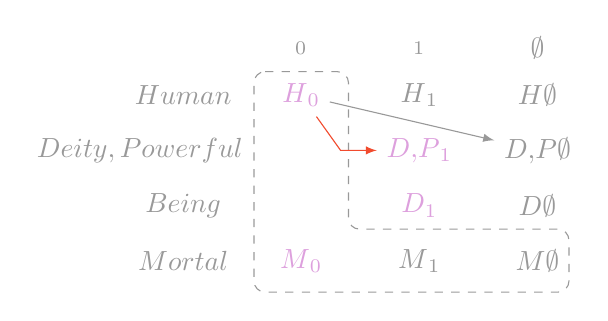
\begin{tikzpicture}
      %\draw[dashed] (1, 3) rectangle (5, 0.3);
  
      \draw[dashed, black!40, rounded corners] (0.9, 3) -- (2.1, 3) -- (2.1,2.3) -- (2.1, 1) -- (4.9, 1) -- (4.9, 0.2) -- (0.9, 0.2) -- cycle;
  
      \node[color=black!40] at (0, 1.3){$\dlFont{Being}$};
      \node[color=black!40] at (0, 2.7){$\dlFont{Human}$};
      \node[color=black!40] at (-0.55, 2){$\dlFont{Deity}, \dlFont{Powerful}$};
      \node[color=black!40] at (0, 0.6){$\dlFont{Mortal}$};
  
      \node[color=black!40] at (1.5,3.3){$\Emc_0$};
      \node[color=black!40] at (3,3.3){$\Emc_1$};
      \node[color=black!40] at (4.5,3.3){$\emptyset$};
      
      \node[Plum] at (3,1.3){$\typel{\dlFont{D}}{\Emc_{1}}$};
      \node[black!40] at (4.5,1.3){$\typel{\dlFont{D}}{\emptyset}$};
  
      \node[Plum] (H2) at (1.5, 2.7){$\typel{\dlFont{H}}{\Emc_{0}}$};
      \node[black!40] (H1) at (3, 2.7){$\typel{\dlFont{H}}{\Emc_{1}}$};
      \node[black!40] (H0) at (4.5, 2.7){$\typel{\dlFont{H}}{\emptyset}$};
  
      %\node[Plum] at (1.5,2){$\typel{\dlFont{D,P}}{\Emc_{0}}$};
      \node[Plum] (DP1) at (3,2){$\typel{\dlFont{D},\!\dlFont{P}}{\Emc_{1}}$};
      \node[black!40] (DP0) at (4.5,2){$\typel{\dlFont{D},\!\dlFont{P}}{\emptyset}$};
  
      \node[Plum] at (1.5,0.6){$\typel{\dlFont{M}}{\Emc_{0}}$};
      \node[black!40] at (3,0.6){$\typel{\dlFont{M}}{\Emc_{1}}$};
      \node[black!40] at (4.5,0.6){$\typel{\dlFont{M}}{\emptyset}$};
  
      %\draw[-latex] (H0) -- (5.5, 2.35) -- (DP0);
      %\draw[-latex] (H1) -- (DP0);
      \draw[-latex, black!40] (H2) -- (DP0);
  
      \node[black!40] at (0.3,3.4){$\footnotesize \ratDom$};

      \draw[-latex, RedOrange] (H2) -- (2,2) -- (DP1);

  \end{tikzpicture} 
    }

  \bigskip \pause

    \begin{itemize}
      \item $\Kmc \models \dlFont{Human} \definc \exists \dlFont{worships}.\dlFont{Anthropomorphic}$ \pause
      \item $\Kmc \not\models \dlFont{Deity} \definc \dlFont{Corporeal}$ (Inheritance Blocking)
    \end{itemize}

\end{frame}

\begin{frame}{Nested Reasoning with Lattice Domains}

  %{\footnotesize\color{red}Obs. ignoring $\dlFont{Human} \definc \exists \dlFont{worships}.\dlFont{Deity}$ axiom.}

  \centering{
  \scalebox{.9}{
        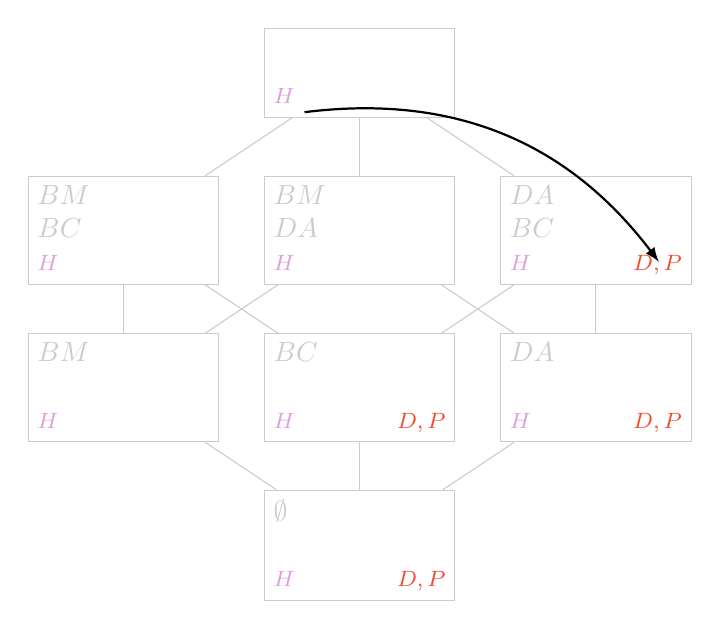
\begin{tikzpicture}
            \node[align=left, draw, color=black!20] at (0,6) (D) {\color{black!20}$\Dmc$  \\ \color{white}$\dlFont{C} \definc \dlFont{F} \hspace{8mm}$ \\ \footnotesize {\color{Plum}$\dlFont{H} \hspace{12mm}$}{ \color{white} $\dlFont{D,P}$}};
          
            %%% Level 2
          
            \node[align=left, draw, color=black!20] at (-3,4) (B1B2) {\color{black!20}$\dlFont{B} \definc \dlFont{M}$  \\ \color{black!20}$\dlFont{B} \definc \dlFont{C} \hspace{8mm}$ \\ \footnotesize {\color{Plum}$\dlFont{H} \hspace{12mm}$}{ \color{white} $\dlFont{D,P}$}};
          
            \node[align=left, draw, color=black!20] at (0,4) (B1P) {\color{black!20}$\dlFont{B} \definc \dlFont{M}$ \\ \color{black!20}$\dlFont{D} \definc \dlFont{A}$ \\ \footnotesize {\color{Plum}$\dlFont{H} \hspace{12mm}$}{ \color{white} $\dlFont{D,P}$}};
          
            \node[align=left, draw, color=black!20] at (3,4) (B2P) {\color{black!20}$\dlFont{D} \definc \dlFont{A} \hspace{8mm}$ \\ \color{black!20}$\dlFont{B} \definc \dlFont{C}$ \\ \footnotesize {\color{Plum}$\dlFont{H} \hspace{12mm}$}{ \color{RedOrange} $\dlFont{D,P}$}};
          
            %%% Level 1
          
            \node[align=left, draw, color=black!20] at (-3,2) (B1) {\color{black!20}$\dlFont{B} \definc \dlFont{M}$  \\ \color{white}$\dlFont{C} \definc \dlFont{F} \hspace{8mm}$ \\\footnotesize {\color{Plum}$\dlFont{H} \hspace{12mm}$}{ \color{white} $\dlFont{D,P}$}};
          
            \node[align=left, draw, color=black!20] at (0,2) (B2) {\color{black!20}$\dlFont{B} \definc \dlFont{C}$ \\ \color{white}$\dlFont{D} \definc \dlFont{I}$ \\ \footnotesize {\color{Plum}$\dlFont{H} \hspace{12mm}$}{ \color{RedOrange} $\dlFont{D,P}$}};
          
            \node[align=left, draw, color=black!20] at (3,2) (P) {\color{black!20}$\dlFont{D} \definc \dlFont{A}$ \\ \color{white}$\dlFont{C} \definc \dlFont{F}$ \\ \footnotesize {\color{Plum}$\dlFont{H} \hspace{12mm}$}{ \color{RedOrange} $\dlFont{D,P}$}};
          
            %%%% Level 0
          
            \node[align=left, draw, color=black!20] at (0,0) (empty) {\color{black!20}$\emptyset$ \\ \color{white}$\dlFont{C} \definc \dlFont{F} \hspace{8mm}$ \\ \footnotesize {\color{Plum}$\dlFont{H} \hspace{12mm}$}{ \color{RedOrange} $\dlFont{D,P}$}};
            
            %%% Lattice lines
            \draw[-, color=black!20] (D)--(B1B2);
            \draw[-, color=black!20] (D)--(B1P);
            \draw[-, color=black!20] (D)--(B2P);
          
            \draw[-, color=black!20] (B1B2)--(B1);
            \draw[-, color=black!20] (B1B2)--(B2);
          
            \draw[-, color=black!20] (B1P)--(B1);
            \draw[-, color=black!20] (B1P)--(P);
          
            \draw[-, color=black!20] (B2P)--(B2);
            \draw[-, color=black!20] (B2P)--(P);
          
            \draw[-, color=black!20] (B1)--(empty);
            \draw[-, color=black!20] (B2)--(empty);
            \draw[-, color=black!20] (P)--(empty);
          
            \draw[-latex, thick, bend left] (-0.7,5.5) to(3.8,3.6);
          
            \end{tikzpicture}
         }
      }
      \begin{itemize}
          \item \footnotesize $\Kmc \models \dlFont{Deity} \definc \dlFont{Corporeal}$ 
          \item \footnotesize $\Kmc \models \dlFont{Human} \definc \exists \dlFont{worships}.\dlFont{Corporeal}$ 
    \end{itemize}
\end{frame}

\begin{frame}{Comparing Different Entailments}
  \centering{
    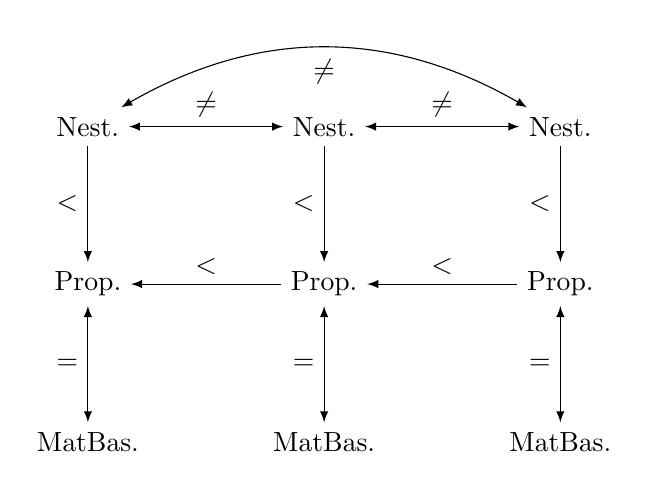
\begin{tikzpicture}
    % % % MatBas
    \node[] at (0,-2) (Mrat) {MatBas. \ratS};
    \node[] at (3,-2) (Mrel) {MatBas. \relS};
    \node[] at (6,-2) (Mlex) {MatBas. \lexS};

    % % % Propositional
    \node[] at (0,0) (Prat) {Prop. \ratS};
    \node[] at (3,0) (Prel) {Prop. \relS};
    \node[] at (6,0) (Plex) {Prop. \lexS};

    % % % Nested
    \node[] at (0,2) (Nrat) {Nest. \ratS};
    \node[] at (3,2) (Nrel) {Nest. \relS};
    \node[] at (6,2) (Nlex) {Nest. \lexS};

    % % % Edges
    \draw [latex-latex](Plex) -- (Mlex) node[midway, left] {$=$};
    \draw [latex-latex](Prel) -- (Mrel) node[midway, left] {$=$};
    \draw [latex-latex](Prat) -- (Mrat) node[midway, left] {$=$};

    \draw [-latex](Plex) -- (Prel) node[midway, above] {$<$};
    \draw [-latex](Prel) -- (Prat) node[midway, above] {$<$};

    \draw [latex-](Plex) -- (Nlex) node[midway, left] {$<$};
    \draw [latex-](Prel) -- (Nrel) node[midway, left] {$<$};
    \draw [latex-](Prat) -- (Nrat) node[midway, left] {$<$};

    \draw [latex-latex](Nlex) -- (Nrel) node[midway, above] {$\not=$};
    \draw [latex-latex](Nrel) -- (Nrat) node[midway, above] {$\not=$};
    \draw [latex-latex, bend right](Nlex) to (Nrat) node[] at(3,2.7) {$\not=$};

    \end{tikzpicture}
    } 
\end{frame}

\begin{frame}{Future work}
\large 
\begin{itemize}
  \item Investigate the complexity of the \strength-entailment for \ELIbot. \pause 
  \item Is it possible to jump from \ELIbot to Horn-$\ALC$ with minor changes to the procedure? \pause 
  \item Investigate what would be needed to go to more expressive Horn-DLs. \pause
  \item TMs to more complex reasoning tasks.
\end{itemize}
\end{frame} 

\begin{frame}
  \centering{
  \includegraphics[scale=.2]{img/flyingpeng.png}
  }

  \centering{Thanks!}
\end{frame}

\end{document}




